% !TEX root = ../intro-stellar-physics.tex

We are now ready to investigate heat transport near the edge, where the optical depth $\tau_{\nu} \lesssim 1$ and photons begin to freely escape. We can no longer use the approximation of radiative diffusion, because conditions in the star are now changing over distances of a mean free path. Let's return to equation~(\ref{e.transfer-equation}) for radiative transport:
\[
	\DD{I_{\nu}}{s} = -\rho\left(\kapabs + \kapscat\right) I_{\nu} + \rho j_{\nu} + \rho\kapscat J_{\nu}.
\]
In general, this is difficult to solve: for some frequencies, the atmosphere will be nearly transparent, while for other frequencies it is quite opaque. Rather than develop the numerical machinery to solve the equation, we shall adopt a few simple approximations (indicated by highlighted bold text in the margins) that will allow us to obtain an approximate solution for the temperature of the stellar atmosphere.

\marginnote[\baselineskip]{\colorbox{yellow}{\textbf{Opacities are gray}}}We assume that the opacity is gray. That is, the opacity is independent of frequency. This is unphysical, but the solutions for temperature and pressure will have the correct overall behavior. Because the opacity is gray, we shall drop the ``$\nu$'' subscript in $\kappa$ and $\tau$.

\begin{exercisebox}[Gray emissivity?]
Does matter with a gray opacity in thermal equilibrium also have a gray emissivity $j_{\nu}$?
\end{exercisebox}

We next define a coordinate system. Since we are in a thin layer near the edge of the star, we will adopt planar coordinates, with $z$ being the altitude above some point. We'll pick $z=0$ to be a point deep enough in the star that $I_{\nu}\approx B_{\nu}$. Then we define the optical depth as
\begin{equation}\label{e.optical-depth-planar}
	\tau = \int_{z}^{\infty} \rho\left(\kappa^{\mathrm{abs}}+\kappa^{\mathrm{sca}}\right)\,\dif z ;
\end{equation}
differentiating this expression gives
\[
	\DD{\tau}{z} = -\rho\left(\kappa^{\mathrm{abs}}+\kappa^{\mathrm{sca}}\right).
\]
Note the ``$-$'': in these coordinates, as $z$ gets larger, $\tau$ gets smaller.

We may rewrite the equation (\ref{e.hydrostatic-equilibrium-g}) of hydrostatic balance as
\begin{eqnarray}
	-\rho g = \DD{P}{z} &=& \DD{P}{\tau}\DD{\tau}{z} = -\rho\kappa,\nonumber\\
	\DD{P}{\tau} &=& \frac{g}{\kappa}.
\label{e.P-tau}
\end{eqnarray}
Since we are in a thin layer, we can take the gravitational acceleration $g$ as being approximately constant. By integrating hydrostatic equilibrium from where $\tau = 0, P = 0$ to where $\tau = 1$, we can get an approximate value of the photospheric pressure,
\[
	P_{\mathrm{ph}} = \int_{0}^{P_{\mathrm{ph}}}\,\dif P = \int_{0}^{1}\frac{g}{\kappa}\,\dif\tau \approx \frac{g}{\kappa}.
\]
\begin{quote}
\emph{The surface gravity sets the pressure at the \textbf{photosphere}, the location where the optical depth is of order unity and where photons can escape from the star.}
\end{quote}

\begin{exercisebox}[Photospheric pressure]
Suppose you observe a star that has a 10\% larger mass and 10\% larger radius than the Sun. All else being equal, how does the pressure at the photosphere of this star compare to that of the Sun?
\end{exercisebox}

\marginnote[\baselineskip]{\colorbox{yellow}{\textbf{Atmosphere is in steady-state LTE}}}
Next, we assume that the matter is in \newterm{local thermal equilibrium} (LTE). This means there is a well-defined temperature at each depth. Furthermore, the emissivity is related to the absorption opacity,
\[
	j_{\nu} = \kappa^{\mathrm{abs}}B_{\nu}.
\]
Note that this does \emph{not} imply anything about the radiation field. We can now take the radiative transfer equation (\ref{e.transfer-equation}) and substitue our definition of optical depth (eq.~[\ref{e.optical-depth-planar}]) to obtain
\begin{equation}\label{e.transfer-gray}
	\mu\DD{I_{\nu}}{\tau} = I_{\nu} - S_{\nu}.
\end{equation}
Here
\[
	S_{\nu} = \frac{j_{\nu} + \kappa^{\mathrm{sca}} J_{\nu}}{\kappa}
	= \frac{\kappa^{\mathrm{abs}} B_{\nu} + \kappa^{\mathrm{sca}} J_{\nu}}{\kappa}.
\]
If, in addition, the matter is in steady-state, then the rate at which energy is absorbed from the radiation field, $\int\kappa^{\mathrm{abs}}I_{\nu}\,\dif\nu\,\dif\Omega$, must equal the rate at which energy is emitted, $\int j_{\nu}\,\dif\nu\,\dif\Omega$. Since we are in LTE,
\[
	\int \left(j_{\nu} - \kappa^{\mathrm{abs}}I_{\nu}\right)\,\dif\nu\,\dif\Omega
	= 4\pi\kappa^{\mathrm{abs}}\int\left(B_{\nu} - J_{\nu}\right)\,\dif\nu = 0.
\]
Since $J = \int J_{\nu}\,\dif\nu = \int B_{\nu}\,\dif\nu = B$, it follows that $S = \int S_{\nu}\,\dif\nu = B$ as well:
\begin{quote}
\emph{For a gray atmosphere in steady-state, local thermal equilibrium, the integrated source function and mean intensity equal the Planck value:}
\[ S(\tau) = J(\tau) = B(\tau), \]
\end{quote}
Note that this does \emph{not} imply that $I_{\nu}=B_{\nu}$ or $J_{\nu}=B_{\nu}$.

We still have the problem that eq.~(\ref{e.transfer-gray}) includes both the derivative and integral of $I_{\nu}$. To get around this, we are going to expand $I_{\nu}$ in Legendre polynomials,
\[
	I_{\nu}(\tau,\mu) = I_{\nu,0}(\tau)\Pl{0}(\mu) + I_{\nu,1}(\tau)\Pl{1}(\mu) + I_{\nu,2}(\tau)\Pl{2}(\mu) + \ldots
\]
and then only include the first two terms, $\Pl{0}(\mu) = 1, \Pl{1} = \mu$. Thus, $I_{\nu}$ is \emph{linear} in $\mu$: $I_{\nu} = I_{\nu,0}(\tau) + I_{\nu,1}(\tau)\mu$. 
\marginnote{\colorbox{yellow}{\textbf{Intensity is linear in $\mu$}}}

In terms of this expansion, the angle-averaged specific intensity is
\[
	J_{\nu}(\tau) = \frac{1}{4\pi}\int I_{\nu}\,\dif\mu\,\dif\phi = I_{\nu,0}(\tau),
\]
and hence the specific energy density is $U_{\nu} = 4\pi/c\cdot J_{\nu} = 4\pi/c\cdot I_{\nu,0}$. The specific flux is
\[
	F_{\nu}(\tau) = \int \mu I_{\nu}\,\dif\mu\,\dif\phi = \frac{4\pi}{3} I_{\nu,1}(\tau).
\]
We can therefore write the intensity as
\begin{equation}
\label{e.intensity-expanded}
I_{\nu}(\tau) = J_{\nu}(\tau) + \frac{3\mu}{4\pi} F_{\nu}(\tau) = \frac{c}{4\pi}U_{\nu}(\tau) + \frac{3\mu}{4\pi} F_{\nu}(\tau).
\end{equation}

\begin{sidebar}[Expansion in Legendre polynomials]
\label{sb.intensity-decomposition}
You may recall from electrostatics that we can decompose the field from a set of charges into a sum of moments: dipole, quadrupole, and so on. The basis functions for this are the Legendre polynomials $\Pl{n}(\cos\theta)$, defined by the expansion
\[
	\frac{1}{\sqrt{1 - 2\mu z + z^{2}}} \equiv \sum_{n=0}^{\infty}\Pl{n}(\mu)z^{n},
\]
for $-1<\mu<1,\;|z| < 1$. The first four polynomials are
\begin{eqnarray*}
	\Pl{0}(\mu) = 1 &\quad& \Pl{2}(\mu) = \frac{1}{2}(3\mu^{2}-1)\\
	\Pl{1}(\mu) = \mu &\quad& \Pl{3}(\mu) = \frac{1}{2}(5\mu^{3}-3\mu),
\end{eqnarray*}
and the first eight Legendre polynomials are plotted below.

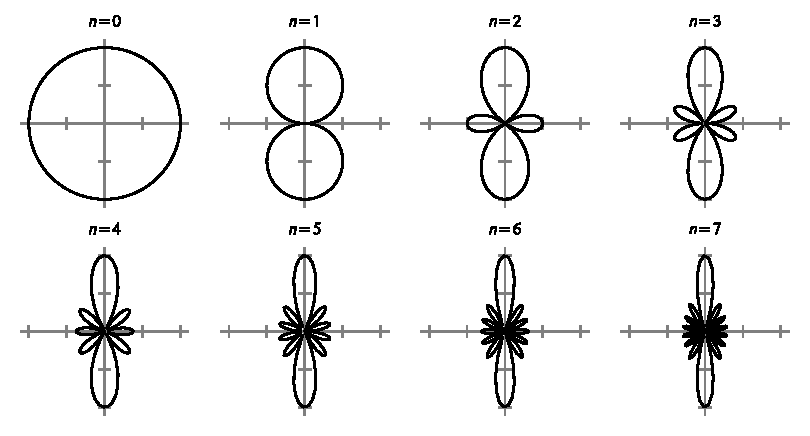
\includegraphics{legendre}

\noindent As $n$ increases, the angular scale of variations becomes finer.

The Legendre polynomials are \emph{orthogonal} in the following sense:
\begin{equation}\label{e.orthogonal}
\int_{-1}^{1}\Pl{n}(\mu)\Pl{m}(\mu)\dif \mu = \left\{
\begin{array}{lr}
	0 &  m\neq n\\
	\frac{2}{2n+1} & m=n
\end{array}\right..
\end{equation}
As a result of this orthogonality, we can decompose the radiative intensity into multipoles:
\begin{equation}\label{e.decomposition}
	I = \sum_{n=0}^{\infty} I_{n} \Pl{n}(\mu).
\end{equation}

\begin{exercisebox}[Odd-even powers of $\mu$]
\label{e.symmetry-powers-mu}
Use eq.~(\ref{e.orthogonal}) to show that $(4\pi)^{-1}\int I\,\dif\Omega = I_{0}$ and $\int \mu I\,\dif\Omega = (4\pi/3)I_{1}$, for $I = I_{0} + I_{1}\mu$.
\end{exercisebox}

\end{sidebar}

Insert the expansion (\ref{e.intensity-expanded}) into the radiative transfer equation (\ref{e.transfer-gray}) and integrate over all angles and frequencies. Since $\tau$ is gray, we can pull the derivative out from the integral,
\begin{eqnarray*}
	\DD{}{\tau}\int \mu I_{\nu}\,\dif\nu\,\dif\Omega &=& \int I_{\nu}\,\dif\nu\,\dif\Omega - \frac{\kappa^{\mathrm{abs}}}{\kappa}\int B_{\nu}\,\dif\nu\,\dif\Omega - \frac{\kappa^{\mathrm{sca}}}{\kappa} \int J_{\nu}\,\dif\nu\,\dif\Omega\\
	\DD{}{\tau}\int F_{\nu}\,\dif\nu &=& \frac{4\pi}{\kappa}\left[
		(\kappa^{\mathrm{abs}}+\kappa^{\mathrm{sca}})\int J_{\nu}\,\dif\nu
		- \kappa^{\mathrm{abs}}\int B_{\nu}\,\dif\nu
		- \kappa^{\mathrm{sca}}\int J_{\nu}\,\dif\nu\right]\\
	\DD{F}{\tau} &=& 4\pi\frac{\kappa^{\mathrm{abs}}}{\kappa}\int\left(J_{\nu}-B_{\nu}\right) = 0.
\end{eqnarray*}
Here we used $\kappa = \kappa^{\mathrm{abs}}+\kappa^{\mathrm{sca}}$ to simplify the right-hand side.

\begin{quote}
\emph{For a steady-state gray atmosphere in local thermal equilibrium, the total flux $F = \int F_{\nu}\,\dif\nu$ is constant.}
\end{quote}
The radiative energy is just passing through. Since the flux at $\tau=0$, outside the star, is $F = \sigmaSB\,\Teff^{4}$, we can substitute that value in our expression for the intensity,
\begin{equation}
\label{e.Inu-expansion}
	I(\mu,\tau) = \frac{c}{4\pi} U(\tau) + \frac{3\mu}{4\pi}\sigmaSB\Teff^{4}.
\end{equation}
To solve for $U_{\nu}(\tau)$, multiply eq.~(\ref{e.transfer-gray}) by $\mu$ and integrate over all angles and frequencies:
\begin{eqnarray}
	\DD{}{\tau}\int\mu^{2}I\,\dif\Omega\,\dif\nu &=& \int\mu I\,\dif\Omega\,\dif\nu
		- \int \mu S\,\dif\Omega\,\dif\nu\nonumber\\
	\frac{c}{4\pi}\DD{}{\tau} \mu^{2}U\,\dif\Omega 
		+ \frac{3}{4\pi}\sigmaSB\Teff^{4}\int\mu^{3}\,\dif\Omega &=& F - \int \mu S\,\dif\Omega\nonumber\\
	\frac{c}{3}\DD{U}{\tau} &=& \sigmaSB\Teff^{4}
\label{e.ODE-U}
\end{eqnarray}
In going from the first to the second line we have used eq.~(\ref{e.Inu-expansion}). In going from the second to the third line, the integrals of $\mu^{3}$ and $\mu S$ vanish because $S$ is independent of angle and $\int_{-1}^{1} \mu\,\dif\mu = \int_{-1}^{1}\mu^{3}\,\dif\mu = 0$. 

Equation~(\ref{e.ODE-U}) is a first-order ODE, which upon integration yields
\begin{equation}\label{e.energy-density-Eddington}
	U(\tau) = \frac{3}{c}F(\tau + \tau_{0}),
\end{equation}
where $\tau_{0}$ is an integration constant. Our intensity is thus
\[
	I(\mu,\tau) = \frac{3}{4\pi}\sigmaSB\Teff^{4}\left(\tau + \tau_{0} + \mu\right).
\]
To fix the integration constant $\tau_{0}$, let's go to where $\tau=0$. Here all of the radiation must be outward-bound. Hence if we integrate $\mu I(\mu,\tau=0)$ over $0\le\mu\le 1$, we should recover the flux:
\[
	\sigmaSB\Teff^{4} = \int_{0}^{2\pi}\int_{0}^{1} \mu I(\mu,\tau=0)\,\dif\mu\,\dif\phi
	= \frac{3}{4}\sigmaSB\Teff^{4}\left(\tau_{0} + \frac{2}{3}\right),
\]
which fixes $\tau_{0} = 2/3$.

To finish this, we note that $J = B$ since we are in steady-state local thermal equilibrium. The radiative energy density is thus $U = (4\pi/c) J = (4\pi/c)B = 4\sigmaSB/c T^{4}$. Substituting this into eq.~(\ref{e.energy-density-Eddington}) then yields
\begin{equation}\label{e.T-tau}
T^{4} = \frac{3}{4}\Teff^{4}\left(\tau + \frac{2}{3}\right).
\end{equation}
This equation, along with eq.~(\ref{e.P-tau}), determines the structure of the stellar atmosphere.

\begin{sidebar}[Decomposition of intensity into moments]
\label{sb.intensity-moments}
It is often useful to describe the intensity in terms of \newterm{moments}. A moment is simply an angle-weighted average of the radiative intensity, where the weight is a power of $\mu$. For example, to take the zeroth-order moment, we multiply $I_{\nu}$ by $\mu^{0}=1$, integrate over all angles, and divide by $4\pi$. This is just the average intensity $J_{\nu} = (4\pi)^{-1}\int I_{\nu}\,\dif\Omega$. To take the first-order moment $H_{\nu}$, we use a weight $\mu^{1}$:
\[
	H_{\nu} = \frac{1}{4\pi}\int_{0}^{2\pi}\int_{-1}^{1}\mu I_{\nu}\,\dif\mu\,\dif\phi.
\]
To take the second-order moment $K_{\nu}$, we use a weight $\mu^{2}$:
\[
	K_{\nu} = \frac{1}{4\pi}\int_{0}^{2\pi}\int_{-1}^{1}\mu^{2} I_{\nu}\,\dif\mu\,\dif\phi.
\]
The first three moments have physically interpretable meanings: the specific radiative energy density, flux, and pressure are $U_{\nu} = (4\pi/c)J_{\nu}$, $F_{\nu} = 4\pi H_{\nu}$, and $P_{\nu} = (4\pi/c) K_{\nu}$, respectively.

By taking moments of the radiative-transfer equation~(\ref{e.transfer-gray}), we reduce the complicated integro-differential equation into a simpler ordinary differential equation. This comes at a cost, however; because the left-hand side contains $\mu\dif/\dif\tau$, the left hand side will have a higher-order moment than the right-hand side. By multiplying eq.~(\ref{e.transfer-gray}) by successively higher powers of $\mu$ and integrating, we will generate an infinite series of ODE's for successively higher moments of $I_{\nu}$.
The trick is to adopt a \newterm{closure relation} that truncates this series. The classic scheme, due to Eddington, is to take $K = J/3$.
The Eddington closure scheme is equivalent to expanding the radiative intensity to terms linear in $\mu$.

\begin{exercisebox}[The Eddington closure scheme]
Show that if we approximate the intensity as $I_{nu}(\mu,\tau) = I_{\nu,0}(\tau) + \mu I_{\nu,1}(\tau)$ (cf.\ eq.~[\ref{e.intensity-expanded}]), then $K_{\nu} = J_{\nu}/3$ identically.
\end{exercisebox}
\end{sidebar}

\begin{exercisebox}[Anisotropy of the intensity]
Deep in the star, we expect the radiation to be nearly isotropic, while it becomes outward-bound as $\tau\to 0$. Let's investigate this. We'll measure the anisotropy of the radiation field using the first two moments of the intensity (Box~\ref{sb.intensity-moments}).
\begin{enumerate}
\item
Demonstrate that $H_{\nu}/J_{\nu} = 0$ if the radiation is isotropic.

\item
Next, suppose the radiation is completely anisotropic: all the photons are headed along precisely the same direction $\mu = 1$. We describe this mathematically as
\begin{equation}
I_{\nu}(\mu) = a_{\nu} \delta(\mu - 1),
\end{equation}
where $\delta(x)$ is the \newterm{Dirac delta function} (see Box~\ref{sb.delta-function}).
Show that $H_{\nu}/J_{\nu} = 1$ for this case.

\item
Now compute $H(\tau)/J(\tau)$ for our gray atmosphere.What is the degree of anisotropy at $\tau = 0$? at $\tau=2/3$? at $\tau = 10$?
\end{enumerate}
\end{exercisebox}

\begin{sidebar}[The Dirac delta function]
\label{sb.delta-function}
The Dirac delta function $\delta(x)$ has the following properties: $\delta(x) = 0, \forall x \neq 0$; and
\[
\int_{-\epsilon}^{\epsilon} \delta(x)\,\dif x = 1.
\]
From this definition, one can show that
\[
	\int f(x) \delta(x-a)\,\dif x = f(a),
\]
where the integral is over any domain containing $x = a$.
\end{sidebar}

%Notice that we can write the weighting factors in terms of Legendre polynomials:
%\begin{eqnarray*}
%	J &=& \frac{1}{4\pi}\int\,\dif\phi\dif\mu\,{\color{red}\mu^{0}}\,I 
%		= \frac{1}{2}\int_{-1}^{1}\dif\mu\sum_{n=0}^{\infty} \,{\color{red}\Pl{0}} I_{n} \\
%	H &=& \frac{1}{4\pi}\int\,\dif\phi\dif\mu\,{\color{red}\mu^{1}}\,I 
%		= \frac{1}{2}\int_{-1}^{1}\dif\mu\sum_{n=0}^{\infty} \,{\color{red}\Pl{1}} I_{n} \\
%	K &=& \frac{1}{4\pi}\int\,\dif\phi\dif\mu\,{\color{red}\mu^{2}}\,I 
%		= \frac{1}{2}\int_{-1}^{1}\dif\mu\sum_{n=0}^{\infty} \,{\color{red} \frac{1}{3}(2\Pl{2}+\Pl{0})} I_{n}
%\end{eqnarray*}
%Now we can use the orthogonality relation (eq.~[\ref{e.orthogonal}]) to compute the integrals:
%\begin{eqnarray*}
%	J &=& I_{0} \\
%	H &=& \frac{1}{3}I_{1} \\
%	K &=& \frac{1}{3}\left(\frac{2}{5}I_{2} + I_{0}\right)
%		= \frac{1}{3}\left(\frac{2}{5}I_{2} + J\right)
%\end{eqnarray*}
%Applying the Eddington approximation, i.e., setting $K = J/3$, means that we must set $I_{2} = 0$. Once we do this, we can solve for $J$, $H$, and $K=J/3$ as functions of optical depth $\tau$. This gives us a description of the radiative intensity in terms of $J(\tau)$ and $H$,
%\[
%	I(\tau,\mu) = J(\tau) + 3H \Pl{1}(\mu) + \cdots \approx J(\tau) + 3H\cos\theta,
%\]
%which neglects the higher order terms $I_{n}\Pl{n},\forall n > 2$.
%\end{sidebar}


